\chapter{\uppercase{Aprendizaje Autom\'{a}tico para la detecci\'{o}n de anomal\'{i}as}}
\label{Capitulo 3}

El t\'{e}rmino Aprendizaje Autom\'{a}tico se refiere a la detecci\'{o}n autom\'{a}tica de patrones significativos dentro de un conjunto de datos \cite{Reference32}. En las \'{u}ltimas d\'{e}cadas se ha convertido en una herramienta com\'{u}n en casi cualquier tarea que requiera la extracci\'{o}n de informaci\'{o}n de gran cantidad de datos, por lo cual se ha convertido en una de las \'{a}reas de m\'{a}s r\'{a}pido crecimiento de la inform\'{a}tica.

\vspace{5mm} %5mm vertical space

Si bien el Aprendizaje Autom\'{a}tico puede resolver algunos problemas que son resueltos con algoritmos tradicionales, ha superado a \'{e}stos en problemas tales como el reconocimiento de im\'{a}genes, voz, lenguaje, escritura, juegos, rob\'{o}tica, an\'{a}lisis de datos, an\'{a}lisis de series de tiempo, etc. Desde esta perspectiva, se espera que mediante la aplicaci\'{o}n del Aprendizaje Autom\'{a}tico se pueda generar un modelo que se ajuste a un comportamiento normal esperado para el agente.

\vspace{5mm} %5mm vertical space

Por lo tanto en este cap\'{i}tulo se detalla las bases te\'{o}ricas necesarias para abordar el desarrollo del m\'{e}todo de detecci\'{o}n de anomal\'{i}as de conducci\'{o}n. En primer lugar, se decribe los diferentes paradigmas de aprendizaje que existen y los diferentes enfoques de modelos, luego, se realiza una descripci\'{o}n del funcionamiento de las redes neuronales y se muestra los diferentes tipos de redes, as\'{i} como tambi\'{e}n se presenta las diferentes t\'{e}cnicas de detecci\'{o}n de anomal\'{i}as que hay y por \'{u}timo se muestra las diferentes m\'{e}tricas de evaluaci\'{o}n que presentan los modelos de aprendizaje autom\'{a}tico. 

\section{Aprendizaje Supervisado, Aprendizaje no Supervisado y Aprendizaje Semi supervisado}
\label{section|aprendizaje}

Existen diversas formas de clasificar los paradigmas de aprendizaje que existen, sin embargo en el presente trabajo s\'{o}lo se tratar\'{a}n el supervisado, el no supervisado y el semi-supervisado.

\subsection{Aprendizaje Supervisado}

El \textbf{Aprendizaje Supervisado} es aquel que cuenta con variables de entrada (X) y una variable de salida (Y), este tipo de aprendizaje utiliza un algoritmo para aprender la funci\'{o}n de mapeo desde la entrada hasta la salida.

\begin{equation}
Y = f(X)
\end{equation}

El objetivo de este tipo de aprendizaje es aproximar la funci\'{o}n de mapeo de tal forma que cuando tenga datos de entrada nuevos (X) pueda predecir las variables de salida (Y) para esos datos. 

\vspace{5mm} %5mm vertical space

Este tipo de aprendizaje aborda dos tipos de problemas: clasificaci\'{o}n y regresi\'{o}n. Los problemas de \textbf{Clasificaci\'{o}n} son aquellos donde la variable de salida es una categor\'{i}a, como por ejemplo: ''Rojo'', ''Azul'', o ''Sano'', ''Enfermo'', por otra parte en los problemas de \textbf{Regresi\'{o}n} la variable de salida es un valor real, tal como: ''precio'' o ''altura''. Algunos de los tipos de problemas m\'{a}s comunes construidos sobre la clasificaci\'{o}n y la regresi\'{o}n incluyen la recomendaci\'{o}n y la predicci\'{o}n de series temporales.

\subsection{Aprendizaje no Supervisado}

Por otro lado el \textbf{Aprendizaje no Supervisado} es aquel donde s\'{o}lo se cuenta con datos de entrada (X) y no hay variables de salida correspondientes, su objetivo principal consiste en modelar la estructura o distribuci\'{o}n subyacente en los datos para aprender m\'{a}s acerca de los mismos.

\vspace{5mm} %5mm vertical space

En cuanto a los problemas del Aprendizaje sin supervisi\'{o}n, pueden ser agrupados en dos: agrupamiento y asociaci\'{o}n. El \textbf{Agrupamiento} es aquel donde se desea descubrir las agrupaciones inherentes en el conjunto de datos, como por ejemplo agrupar clientes por comportamiento de compra. Por otra parte la \textbf{Asociaci\'{o}n} es aquella que desea descubrir reglas que describen grandes porciones de sus datos, por ejemplo las personas que compran X tambi\'{e}n tienden a comprar Y. Algunos de los algoritmos de aprendizaje sin supervisi\'{o}n m\'{a}s populares son: K-means (para problemas de agrupamiento) y algoritmo Apriori (para problemas de aprendizaje de reglas de asociaci\'{o}n).

\subsection{Aprendizaje Semi-Supervisado}

Por \'{u}ltimo se encuentra el \textbf{Aprendizaje Semi-supervisado}, el cual abarca aquellos problemas donde se tiene gran cantidad de datos de entrada (X) y s\'{o}lo algunos de los datos est\'{a}n etiquetados (Y). Este tipo de problemas se encuentran entre el aprendizaje supervisado y el no supervisado, adem\'{a}s es importante se\~{n}alar que muchos de los problemas de Aprendizaje Autom\'{a}tico en el mundo real se encuentran en esta \'{a}rea, esto debido a que resulta costoso o puede requerir mucho tiempo etiquetar el conjunto de datos, mientras que los datos no etiquetados son baratos, adem\'{a}s de ser f\'{a}ciles de recolectar y almacenar. Este tipo de problemas pueden usar una combinaci\'{o}n de t\'{e}cnicas supervisadas y no supervisadas para ser resueltos.

\vspace{5mm} %5mm vertical space

Dado que los m\'{e}todos de Aprendizaje Supervisado requieren una gran cantidad de datos de entrenamiento etiquetados, es importante aclarar que la recolecci\'{o}n de muestras negativas (conducci\'{o}n an\'{o}mala) es d\'{i}ficil y riesgosa para este estudio en particular; adem\'{a}s el enfoque supervisado presenta una limitaci\'{o}n potencial, la cual es: la detecci\'{o}n de nuevos patrones at\'{i}picos, esto debido a que el modelo resultante s\'{o}lo esta entrenado para reconocer un conjunto limitado de patrones an\'{o}malos, por lo cual al momento en que se presente un nuevo patr\'{o}n este modelo ser\'{a} incapaz de reconocerlo.

\vspace{5mm} %5mm vertical space

Por otra parte el enfoque sin supervisi\'{o}n tiene la ventaja de no requerir informaci\'{o}n etiquetada, sin embargo a menudo sufre altas tasas de falsas alarmas y bajas tasas de detecci\'{o}n \cite{Reference33}. 

\vspace{5mm} %5mm vertical space

En muchas aplicaciones, incluyendo la del presente estudio, los ejemplos normales son f\'{a}ciles de conseguir, mientras que los an\'{o}malos son bastante dif\'{i}ciles de obtener, en consecuencia, para la realizaci\'{o}n de este estudio, se ha optado por la aplicaci\'{o}n del enfoque Semi-supervisado. De esta manera, como se mencion\'{o} en el Cap\'{i}tulo \ref{Capitulo 2}, el enfoque de \textbf{detecci\'{o}n de anomal\'{i}as Semi-supervisado} s\'{o}lo dispone de muestras normales en el conjunto de entrenamiento; es decir, no se puede obtener informaci\'{o}n sobre anomal\'{i}as, por lo tanto las muestras desconocidas se clasifican como valores at\'{i}picos, siempre y cuando su comportamiento sea muy diferente al de las muestras normales ya conocidas.

\vspace{5mm} %5mm vertical space

Como se mencion\'{o} en esta secci\'{o}n todos estos enfoques de aprendizaje se basan en generar un \textbf{Modelo} capaz de ayudar ya sea en tareas de clasificaci\'{o}n, agrupaci\'{o}n, etc; sin embargo existe m\'{a}s de un tipo de modelos. En la siguiente secci\'{o}n se detallar\'{a} en profundidad los diferentes tipos de modelos que existen.

%%%%%%%%%%%%%%%%

\section{Modelos Generativos y Discriminativos}

Cuando se utiliza Aprendizaje Autom\'{a}tico existen dos principales enfoques para entender (modelar) el mundo real y tomar decisiones. Estos dos enfoques son los modelos discriminativos y generativos. M\'{a}s formalmente los modelos generativos y discriminativos representan dos distintas estrategias para estimar la probabilidad que un objeto en particular pertenece a una categor\'{i}a \cite{Reference42}.

%Es cierto y correcto, pero quisiera que explicaras la diferencia entre un modelo generativo y uno discriminativo ya que no es lo mismo y si solo dices esto se puede pensar que solo intentas capturar una distribución y nada más.

\vspace{5mm} %5mm vertical space

Los \textbf{modelos discriminativos} se basan en la probabilidad condicionada $P(Y|X)$, es decir, aprenden un mapa directo de un conjunto de caracter\'{i}sticas \textit{X} a etiquetas de clases \textit{Y}. Este tipo de modelos intentan modelar simplemente dependiendo de los datos observados (conjunto de datos), adem\'{a}s hacen menos suposiciones sobre las distribuciones; sin embargo dependen en gran medida de la calidad de los datos. Algunos ejemplos de modelos discriminativos son: Regresi\'{o}n Log\'{i}stica, SVM (Support Vector Machine - M\'{a}quina de vectores de soporte), Redes Neuronales, Random Forest, entre otros.

\vspace{5mm} %5mm vertical space

Por otra parte los \textbf{modelos generativos} apuntan a una descripci\'{o}n probabil\'{i}stica completa del conjunto de datos, su objetivo es desarrollar la distribuci\'{o}n de probabilidad conjunta P(X,Y), ya sea directamente o calculando $P(Y|X)$ y $P(X)$, para luego inferir las probabilidades condicionadas requeridas para clasificar nuevos datos. Estos modelos ayudan a especificar la incertidumbre de un modelo, algunos ejemplos de modelos generativos son: Gaussian Mixture Model, Hiden Markov Model, Restricted Bolzmann Machine, Generative Adversial Networks (GAN), entre otros.

\vspace{5mm} %5mm vertical space

Los modelos discriminativos han estado a la vanguardia del éxito del Aprendizaje Automático en los \'{u}ltimos a\~{n}os, ya que estos modelos hacen predicciones que dependen de una entrada dada, aunque no puedan generar nuevas muestras o datos, por lo que en el presente estudio se dar\'{a} preferencia al uso de modelos discriminativos.

\vspace{5mm} %5mm vertical space

A continuaci\'{o}n se realizar\'{a} un repaso de las bases te\'{o}ricas fundamentales de algunas t\'{e}cnicas del Aprendizaje Semi-Supervisado con un enfoque discriminativo, para posteriormente detallar que tipo de algoritmos se aplicar\'{a} en el m\'{e}todo propuesto en este trabajo de investigaci\'{o}n.

\section{Redes Neuronales Artificiales}

La Red Neuronal Artificial o ANN\footnote{\textbf{ANN}, Artificial Neural Network (Red Neuronal Artificial)} es un paradigma de procesamiento de informaci\'{o}n inspirado en la manera en la que el sistema nervioso biol\'{o}gico procesa la informaci\'{o}n. Se compone de una gran cantidad de elementos de procesamiento (neuronas) altamente interconectados que trabajan al un\'{i}sono para resolver un problema espec\'{i}fico.

\subsection{Neuronas o nodos}

Las \textbf{neuronas biol\'{o}gicas} (c\'{e}lulas nerviosas) son las unidades fundamentales del cerebro y del sistema nervioso. Las neuronas son las c\'{e}lulas responsables de recibir informaci\'{o}n sensorial del mundo externo a trav\'{e}s de las dendritas, procesarla y dar una salida a trav\'{e}s del ax\'{o}n (Ver Figura \ref{fig:neurona}). 

 \begin{figure}[h!]
  \begin{center}	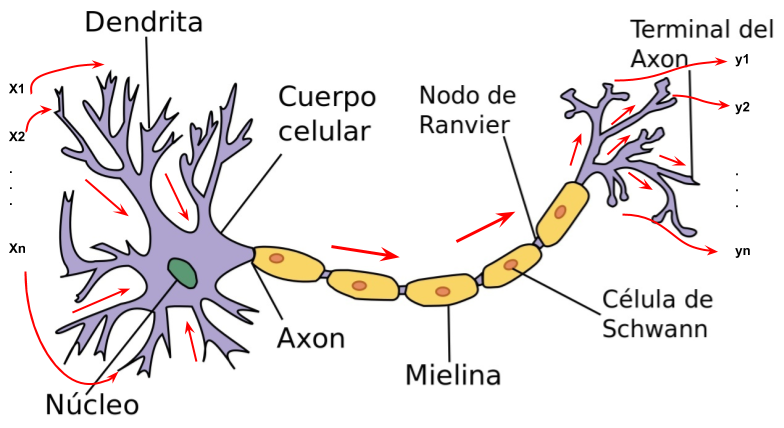
\includegraphics[width=0.95\textwidth, frame]{imagenes/Cap4/neurona}
  \caption{Gr\'{a}fico de una neurona biol\'{o}gica. Reproducido desde \protect\cite{Reference67}.}
  \label{fig:neurona}
  \end{center}
\end{figure}

Una neurona cerebral puede recibir unas 10000 entradas y enviar a su vez su salida a cientas de neuronas.

\vspace{5mm} %5mm vertical space

La conexi\'{o}n entre neuronas se llama \textbf{sinapsis}, esta no es una conexi\'{o}n f\'{i}sica, sino que existe 2 mm. de separaci\'{o}n entre neronas. Estas conexiones son unidireccionales, donde la transmisi\'{o}n de la informaci\'{o}n se hace de forma el\'{e}ctrica en el interior de la neurona  y de forma qu\'{i}mica entre neuronas, gracias a los neurotransmisores.

\vspace{5mm} %5mm vertical space

Una \textbf{neurona artificial} es un procesador elemental, debido a que procesa un vector $x(x_{1},x_{2}, ... ,x_{n})$ de entradas y produce una respuesta o salida \'{u}nica. Los elementos principales de una neurona artificial son los siguientes:

\begin{figure}[h!]
  \begin{center}	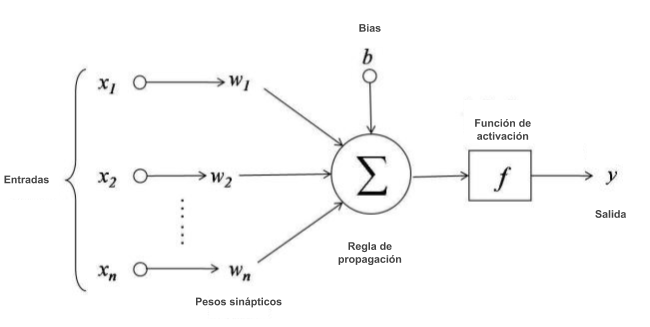
\includegraphics[width=0.95\textwidth, frame]{imagenes/Cap4/neurona_artificial}
  \caption{Gr\'{a}fico de una neurona artificial. Reproducido desde \protect\cite{Reference68}.}
  \label{fig:neurona}
  \end{center}
\end{figure}

\begin{itemize}
\item \textbf{Las entradas} que reciben los datos de otras neuronas, estas entradas ser\'{i}an las dendritas de una neurona biol\'{o}gica.
\item \textbf{Los pesos sin\'{a}pticos $w_{ij}$}. En una neurona artificial a aquellas entradas que vienen de otras neuronas se les asigna un peso (factor de importancia). Este peso es un valor num\'{e}rico que se modifica durante el proceso de entrenamiento de una red neuronal, y por lo tanto es aqu\'{i} donde se almacena la informaci\'{o}n que hace que la red sirva para un prop\'{o}sito u otro.
\item \textbf{Regla de propagaci\'{o}n}. Con las entradas y los pesos sin\'{a}pticos, se suele hacer alg\'{u}n tipo de operaci\'{o}n para obtener el valor potencial postsin\'{a}ptico; una de las operaciones m\'{a}s comunes es sumar las entradas, pero teniendo en cuenta la importancia (peso sin\'{a}ptico) de cada una; esta operaci\'{o}n se llama \textit{suma ponderada} \ref{eqn:suma_pon}, sin embargo otras operaciones tambi\'{e}n son posibles. Otra regla de propagaci\'{o}n que es habitual es la distancia euclidea.
\begin{equation}
h_{i}(t) = \sum_{j}{w_{ij}x_{j}}
\label{eqn:suma_pon}
\end{equation}
\item \textbf{Funci\'{o}n de activaci\'{o}n}. El valor obtenido con la regla de propagaci\'{o}n, se filtra a trav\'{e}s de una funci\'{o}n conocida como \textit{funci\'{o}n de activaci\'{o}n} y es la que da la salida de la neurona. La función de activación es importante debido a que es la que decide si una neurona debe activarse o no, adem\'{a}s si esta función no se aplica la señal de salida de la neurona sería simplemente una función lineal.
\end{itemize}

\subsection{Tipos de funciones de activaci\'{o}n}

Existen diferentes funciones de activaci\'{o}n, a continuaci\'{o}n solo se presentar\'{a} las m\'{a}s usadas en el \'{a}mbito de las redes neuronales.

\begin{figure}
        \centering
        \fbox{\begin{varwidth}{\textwidth}
        
        \centering
        \begin{subfigure}[h]{0.45\textwidth} 
            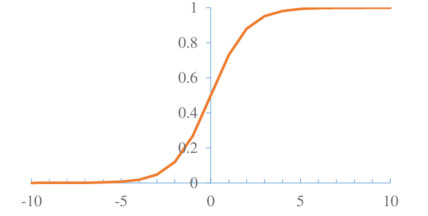
\includegraphics[width=\textwidth]{imagenes/Cap4/sigmoid}
            \caption{Funci\'{o}n Sigmoide}
            \label{fig:sigmoid}
        \end{subfigure}       
        \begin{subfigure}[h]{0.45\textwidth} 
            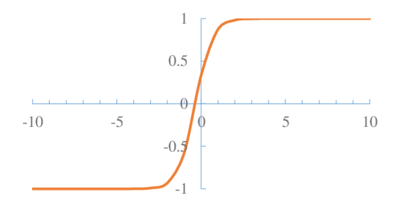
\includegraphics[width=\textwidth]{imagenes/Cap4/tanh}
            \caption{Funci\'{o}n Tanh}
            \label{fig:tanh}
        \end{subfigure}
        
        \begin{subfigure}[h]{0.45\textwidth} 
            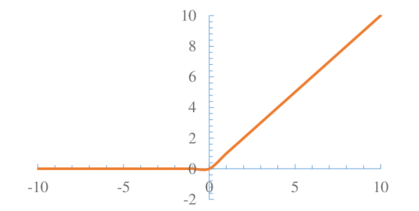
\includegraphics[width=\textwidth]{imagenes/Cap4/relu}
            \caption{Funci\'{o}n ReLU}
            \label{fig:relu}
        \end{subfigure}       
        \begin{subfigure}[h]{0.45\textwidth} 
            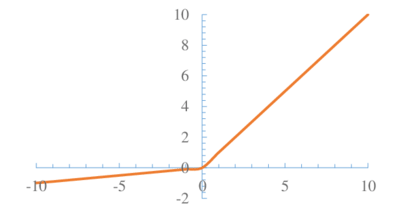
\includegraphics[width=\textwidth]{imagenes/Cap4/l_relu}
            \caption{Funci\'{o}n Leaky ReLu}
            \label{fig:l_relu}
        \end{subfigure}
        \begin{subfigure}[h]{0.45\textwidth} 
            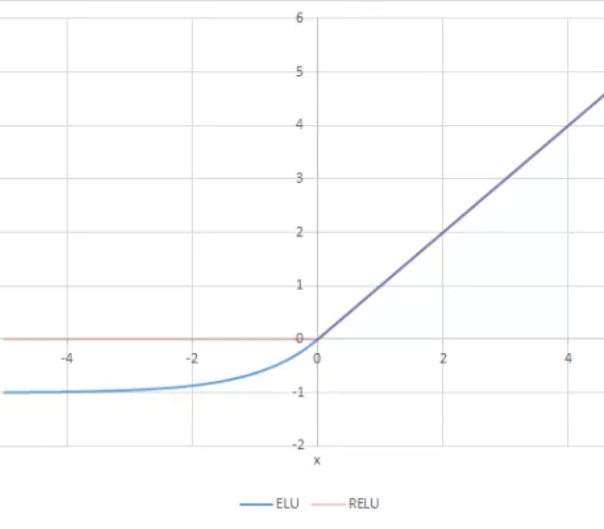
\includegraphics[width=\textwidth]{imagenes/Cap4/elu}
            \caption{Funci\'{o}n ELU}
            \label{fig:elu}
        \end{subfigure}
        \end{varwidth}}
        \caption{Funciones de activaci\'{o}n \protect\cite{Reference69}.}
        
		\label{fig:funciones_activacion}
    \end{figure}
    
\subsubsection{Funci\'{o}n de activaci\'{o}n sigmoide (funci\'{o}n log\'{i}stica)}

Una funci\'{o}n sigmoide es una funci\'{o}n matem\'{a}tica que tiene una curva caracter\'{i}stica en forma de ''S'' o una curva sigmoidea que oscila entre 0 y 1 (Ver Figura \ref{fig:sigmoid}), por lo que esta funci\'{o}n suele ser utilizada en modelos donde se necesita predecir una probabilidad como una salida. Esta funci\'{o}n viene definida por siguiente f\'{o}rmula:

\begin{equation}
f(x) = \frac{1}{1+e^{-x}}
\end{equation}

La funci\'{o}n sigmoide se aplic\'{o} con éxito en problemas de clasificación binaria, modelado de tareas de regresión logística, así como otros dominios de red neuronal, sin embargo, sufre inconvenientes importantes que incluyen gradientes húmedos agudos durante la propagación hacia atrás desde capas ocultas más profundas a las capas de entrada, saturación de gradiente, convergencia lenta y salida no centrada en cero, lo que hace que las actualizaciones de gradiente se propaguen en diferentes direcciones.

\subsubsection{Funci\'{o}n de tangente hiperb\'{o}lica - tanh}

Es bastante similar a Sigmoid pero tiene un rendimiento mucho mejor respecto al entrenamiento de redes neuronales multicapa, su naturaleza es no lineal. \'{E}sta funci\'{o}n est\'{a} centrada en 0 y su rango se encuentra entre -1 y 1 (Ver Figura \ref{fig:tanh}), por lo tanto, su salida esta definida por:

\begin{equation}
f(x)=\frac{e^{x}-e^{-x}}{e^{x}+e^{-x}}
\end{equation}
    
Aunque esta funci\'{o}n tenga un mejor rendimiento que la sigmoide, no pudo resolver el problema de gradiente de fuga que tienen las funciones sigmoideas. Una de las principales ventajas de la funci\'{o}n tangencial es que produce una salida centrada a cero, lo cual ayuda al proceso de propagaci\'{o}n hacia atr\'{a}s.

\vspace{5mm} %5mm vertical space

Las funciones de tangente se han utilizado principalmente en redes neuronales recurrentes para el procesamiento del lenguaje natural \cite{Reference43} y tareas de reconocimiento del habla \cite{Reference44}.
    
\subsubsection{Funci\'{o}n de unidad lineal rectificada (Rectified Linear Unit - ReLU)}

La funci\'{o}n ReLU fue propuesta por Nair y Hinton en 2010, y desde entonces ha sido la funci\'{o}n de activaci\'{o}n m\'{a}s ampliamente utilizada para aplicaciones de aprendizaje autom\'{a}tico con redes neuronales. ReLU es una funci\'{o}n de activaci\'{o}n de aprendizaje m\'{a}s r\'{a}pido \cite{Reference46}, por lo que demostr\'{o} ser la funci\'{o}n m\'{a}s exitosa y m\'{a}s usada. Esta funci\'{o}n ofrece un mejor rendimiento y generalizaci\'{o}n que las funciones sigmoide y tangente en el aprendizaje con redes neuronales.

\vspace{5mm} %5mm vertical space

ReLU representa una función casi lineal y, por lo tanto, conserva las propiedades de los modelos lineales que lo hace fácil de optimizar, con métodos de descenso de gradiente.

\vspace{5mm} %5mm vertical space

La función de activación de ReLU realiza una operación de umbral para cada elemento de entrada donde los valores inferiores a cero se establecen en cero (Ver Figura \ref{fig:relu}), por lo que ReLU esta definida por:

\begin{equation}
f(x) = max(0,x) = \left\lbrace
\begin{array}{ll}
\textup{si } x_{i}\geq0 & x_{i}\\
\textup{si } x_{i} < 0 & 0
\end{array}
\right.
\end{equation}

Esta función rectifica los valores de las entradas inferiores a cero, obligándolos a convertirse en cero, con lo cual elimina el problema de gradiente de fuga observado en los tipos anteriores de función de activación. La función ReLU se ha usado dentro de las unidades ocultas de las redes neuronales.

\vspace{5mm} %5mm vertical space

La principal ventaja de utilizar ReLU es que garantiza un cálculo más rápido, ya que no calcula exponenciales y divisiones, con una velocidad general de cálculo mejorada \cite{Reference45}. Otra propiedad de ReLU es que introduce la escasez en las unidades ocultas, ya que reduce los valores entre cero y máximo. Sin embargo, ReLU tiene la limitación de que se sobreajusta fácilmente en comparación con la función sigmoidea, aunque se ha adoptado la técnica de abandono para reducir el efecto de sobreajuste de ReLU y las redes rectificadas mejoraron el rendimiento de las redes neuronales.

\vspace{5mm} %5mm vertical space

ReLU tiene una limitación significativa de que a veces es frágil durante el entrenamiento, causando la muerte de algunos de los gradientes. Esto hace que algunas neuronas también estén muertas, para resolver los problemas de neuronas muertas, se propuso la funci\'{o}n de activaci\'{o}n Leaky ReLU.

\subsubsection{Leaky ReLU (LReLU)}

Fue propuesta el a\~{n}o 2013 como una funci\'{o}n de activaci\'{o}n, esta funci\'{o}n introduce una peque\~{n}a pendiente negativa a ReLU para mantener y mantener vivas las actualizaciones de peso durante el proceso de propagaci\'{o}n \cite{Reference44}. El par\'{a}metro $\alpha$ fue introducido como una soluci\'{o}n a los problemas de neuronas muertas de ReLU. Esta funci\'{o}n calcula el gradiente con un valor constante muy peque\~{n}o para el gradiente negativo $\alpha$ en el rango de 0.01, por lo que LReLU (Ver Figura \ref{fig:l_relu}) se calcula como:

\begin{equation}
f(x) = \alpha x + x = \left\lbrace
\begin{array}{ll}
\textup{si } x_{i}>0 & x_{i}\\
\textup{si } x_{i} \leq 0 & \alpha x_{i}
\end{array}
\right.
\end{equation}

\subsubsection{Funci\'{o}n de Unidad Lineal Exponencial (ELU)}

La funci\'{o}n ELU\footnote{\textbf{ELU, }Exponencial Lineal Unit} tiende a converger el costo a cero m\'{a}s rapido y produce resultados m\'{a}s precisos. A diferencia de otras funciones de activaci\'{o}n ELU tiene una constante alfa adicional que deber\'{i}a ser un n\'{u}mero positivo.

\vspace{5mm} %5mm vertical space

Es muy similar a ReLU ya que ambas tienen una funci\'{o}n identidad para las entradas positivas, sin embargo en las entradas negativas ELU se suaviza lentamente hasta que su salida es igual $-\alpha$ mientras que en ReLU se suaviza bruscamente. La funci\'{o}n ELU se calcula seg\'{u}n la ecuaci\'{o}n \ref{eqn:elu}.

\begin{equation}
f(x) = \left\lbrace
\begin{array}{ll}
\textup{si } x_{i}>0 & x_{i}\\
\textup{si } x_{i} \leq 0 & \alpha *( e^{x_{i}}-1)
\end{array}
\right.
\label{eqn:elu}
\end{equation}

\subsection{Arquitectura de las Redes Neuronales}

Una red neuronal regular consiste de una cadena de capas interconectadas de neuronas, estas capas son: una capa de entrada, una o varias capas ocultas y una capa de salida. 

\begin{figure}[h!]
  \begin{center}	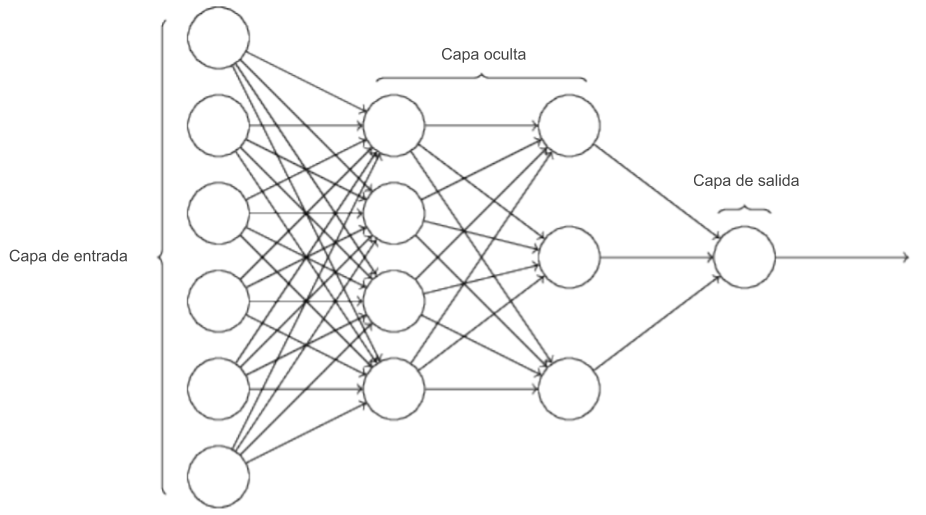
\includegraphics[width=0.95\textwidth, frame]{imagenes/Cap4/arquitectura}
  \caption{Arquitectura de una neurona artificial. Reproducido desde \protect\cite{Reference70}.}
  \label{fig:arquitectura}
  \end{center}
\end{figure}

La figura \ref{fig:arquitectura} es un ejemplo de una red neuronal muy simple; en esta figura la capa m\'{a}s a la izquierda se llama \textbf{capa de entrada}, y las neuronas dentro de esta capa se llaman neuronas de entrada. La capa m\'{a}s a la derecha o de \textbf{salida} contiene las neuronas de salida. Y por \'{u}ltimo las dos capas intermedias son las \textbf{capas ocultas} de la red neuronal, estas se llaman as\'{i} debido a que las neuronas de esta capa no son de entrada o de salida; una red neuronal puede tener una o m\'{a}s capas ocultas.

\vspace{5mm} %5mm vertical space

A diferencia del cerebro humano, una Red Neuronal Artificial tiene una estructura predefinida bastante estricta, las conexiones entre neuronas son siempre hacia adelante (feedforward): las conexiones van desde las neuronas de una determinada capa hacia las neuronas de la siguiente capa, es decir, no existen conexiones laterales ni conexiones hacia atr\'{a}s. Esto significa que una neurona que fue activada en la capa 3 no puede activar a una neurona de la capa 2 o anterior.

\subsection{Proceso de aprendizaje de las Redes Neuronales}

Una caracter\'{i}stica clave de las  redes neuronales es su proceso de aprendizaje iterativo, es decir, cada ejemplo del conjunto de entrenamiento se presenta a la red, uno a la vez, con lo que los pesos asociados con los valores de entrada se ajustan cada vez. Durante esta fase de aprendizaje, la red se entrena ajustando los pesos para predecir una salida correcta para las muestras de entrada.

\vspace{5mm} %5mm vertical space

Las redes neuronales tienen la ventaja de tener una alta tolerancia a los datos ruidosos, como tambi\'{e}n una alta capacidad para clasificar patrones con los que no han sido entrenados. La t\'{e}cnica de entrenamiento de redes neuronales m\'{a}s popular es el \textbf{algoritmo de retropropagaci\'{o}n} (Backpropagation). 

\vspace{5mm} %5mm vertical space

Una vez que se define la estructura de una red para una aplicaci\'{o}n en particular, est\'{a} lista para ser capacitada. Para comenzar este proceso, los pesos iniciales se eligen al azar, para luego proceder con el entrenamiento (aprendizaje). 

\subsubsection{Backpropagation}

Una red neuronal propaga la se\~{n}al de los datos de entrada hacia adelante a trav\'{e}s de sus par\'{a}metros en el momento de la decisi\'{o}n; para luego propagar hacia atr\'{a}s la informaci\'{o}n sobre el error, para que se pueda alterar los par\'{a}metros. Esto sucede siguiendo los siguientes pasos:

\begin{itemize}
\item La red adivina los datos de salida, usando sus par\'{a}metros.
\item La red mide su precisi\'{o}n con una funci\'{o}n de p\'{e}rdida.
\item El error es propagado hacia atr\'{a}s para ajustar los par\'{a}metros equivocados.
\end{itemize}

Por lo tanto se puede decir que el algoritmo de Backpropagation toma el error asociado con una suposición errónea por parte de la red neuronal, y usa ese error para ajustar los parámetros de la red neuronal en la dirección que genere un menor error.

\section{Tipos de Redes Neuronales}

\subsection{Autoencoders}

Un Autoencoder es una Red Neuronal Artificial usada para aprendizaje autom\'{a}tico no supervisado, esta entrenada para reconstruir sus propias entradas, es decir, predecir el valor de la salida $\hat{x}$ dada una entrada $x$ v\'{i}a una capa oculta $h$, ver Figura \ref{fig:autoencoder1}. Los autoencoders suelen ser usados para reducci\'{o}n de dimensionalidad y aprendizaje de caracter\'{i}sticas. 

\begin{figure}[h!]
  \begin{center}	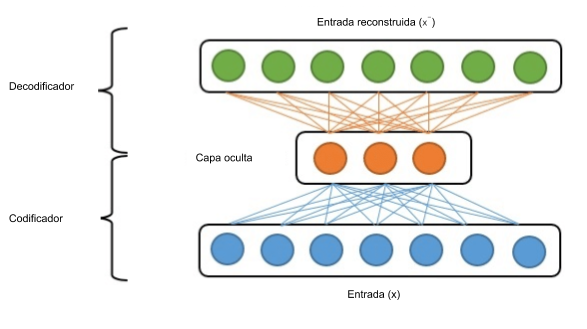
\includegraphics[width=0.95\textwidth, frame]{imagenes/Cap4/autoencoder}
  \caption{Gr\'{a}fico de un Autoencoder (Elaboraci\'{o}n propia).}
  \label{fig:autoencoder1}
  \end{center}
\end{figure}

Los autoencoders est\'{a}n compuestos de dos partes: el codificador y decodificador. El codificador aprende una representaci\'{o}n compresa de los datos de entrada, este puede ser definido con la funci\'{o}n de codificaci\'{o}n $h=encoder(x)$, el cual es definido por una funci\'{o}n lineal o no lineal. Si la funci\'{o}n del codificador es no lineal el autoencoder ser\'{a} capaz de aprender m\'{a}s caracter\'{i}sticas que un PCA lineal. El prop\'{o}sito del decodificador es reconstruir su propia entrada v\'{i}a la funci\'{o}n de decodificaci\'{o}n, $\hat{x} = decodificador(h)$.

\vspace{5mm} %5mm vertical space

La diferencia entre la entrada y la entrada reconstruida es el \textbf{error de reconstrucción}. Durante el entrenamiento, el autoencoder minimiza el error de reconstrucción como una función objetivo. Los autoencoders se usan a menudo para la generación de datos como modelos generativos. El decodificador de un autoencoder puede generar una salida dada una representación comprimida asignada artificialmente.

\subsection{Redes neuronales convolucionales}

Para algunos tipos de datos, especificamente para im\'{a}genes, las redes neuronales convencionales no est\'{a}n bien adaptadas; lo cual conlleva que en el estudio \citeA{Reference48} propongan las redes neuronales convolucionales (CNN\footnote{\textbf{CNN,} Convolutional Neural Network}) para solucionar ese problema. Las CNN han revolucionado el procesamiento de im\'{a}genes y han eliminado la extracci\'{o}n manual de caracter\'{i}sticas. Una CNN act\'{u}a directamente en matrices, o incluso en tensores para im\'{a}genes con tres canales de color RGB; por lo que actualmente, las CNN se usan ampliamente para la clasificaci\'{o}n de im\'{a}genes, reconocimiento de objetos, reconocimiento de rostros, entre otros.

\vspace{5mm} %5mm vertical space

Las CNN no solo brindan un mejor rendimiento en comparaci\'{o}n con otros algoritmos de detecci\'{o}n; sino que incluso en algunos casos superan a los humanos, como por ejemplo en la clasificaci\'{o}n de objetos en categor\'{i}as espec\'{i}ficas como la raza particular de un perro o una especie de ave \cite{Reference49}.

\vspace{5mm} %5mm vertical space

Al apilar múltiples y diferentes capas en una CNN, se crean arquitecturas complejas para los problemas de clasificación. Los cuatro tipos de capas que son más comunes son: capa de convolución, capa de agrupación/submuestreo, capa no lineal y capa completamente conectada. En la Figura \ref{fig:cnn} se puede ver un ejemplo de una CNN, donde la primera y tercera capa son capas convolucionales, la segunda y la cuarta son capas de submuestreo y por \'{u}ltimo la quinta y la sexta capa con capas completamente conectadas. 

\begin{figure}[h!]
  \begin{center}	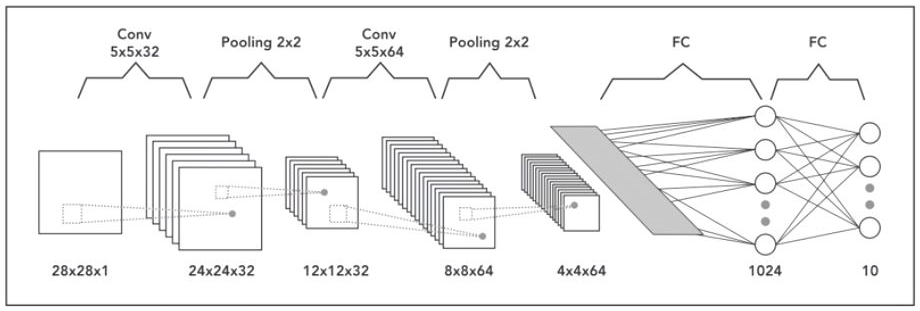
\includegraphics[width=0.95\textwidth]{imagenes/Cap4/cnn}
  \caption{Arquitectura de una Red Neuronal Convolucional (CNN) \protect\cite{Reference71}.}
  \label{fig:cnn}
  \end{center}
\end{figure}

\subsection{Redes neuronales recurrentes}

Para entender la importancia de las series de tiempo se puede tomar la siguiente analog\'{i}a, los seres humanos no comienzan a pensar desde cero cada segundo, por lo que al leer un documento se comprende cada palabra bas\'{a}ndose en la comprensi\'{o}n de las palabras anteriores, es decir, no se elimina todo y se empieza a pensar de cero cada vez, dada \'{e}sta afirmaci\'{o}n se puede decir que los pensamientos de los seres humanos tienen persistencia.

\vspace{5mm} %5mm vertical space

Las redes neuronales tradicionales no tienen persistencia de los datos, lo que para algunos problemas en concreto, incluyendo el que se aborda en este trabajo, es una gran deficiencia. Con el fin de resolver este tipo de problemas aparecen las Redes Neuronales Recurrentes (RNN\footnote{\textbf{RNN,} Recurrent Neural Network}), las cuales son un tipo de red neuronal artificial propuesta en los a\~{n}os 80 (\citeNP{Reference34}; \citeNP{Reference35}; \citeNP{Reference36}) dise\~{n}ada para reconocer patrones en secuencias de datos, como texto, genomas, escritura a mano, datos de series de tiempo num\'{e}ricos que emanan de sensores, entre otros.

\vspace{5mm} %5mm vertical space

Las RNN son una familia particular de redes neuronales donde la red contiene una o más conexiones de retroalimentación, de modo que la activación de un grupo de neuronas puede fluir en un bucle. Esta propiedad hace que el modelo pueda retener informaci\'{o}n sobre el pasado, lo que le permite descubrir correlaciones temporales entre eventos que est\'{a}n muy lejos unos de otros en los datos.

\vspace{5mm} %5mm vertical space

Las RNN tienen una cierta memoria de lo que sucedi\'{o} anteriormente en una secuencia de datos, esto ayuda al sistema a ganar contexto de los datos. Te\'{o}ricamente se dice que las RNN tiene memoria infinita, es decir, este tipo de redes tienen la capacidad de mirar hacia atr\'{a}s indefinidamente; sin embargo en la pr\'{a}ctica s\'{o}lo se puede mirar atr\'{a}s unos \'{u}ltimos pasos.

\begin{figure}[h!]
  \begin{center}	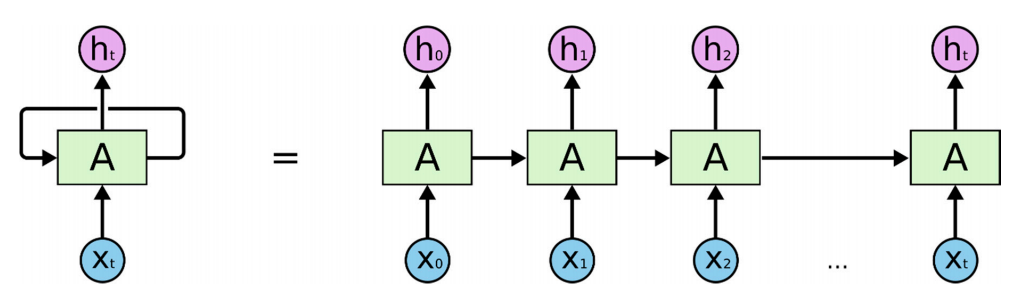
\includegraphics[width=0.95\textwidth, frame]{imagenes/Cap4/rnn}
  \caption{Procesamiento secuencial en una red neuronal recurrente (RNN) \protect\cite{Reference53}.}
  \label{fig:rnn}
  \end{center}
\end{figure}

En la Figura \ref{fig:rnn} se ilustra una simple RNN con una unidad de entrada, una unidad de salida y una unidad oculta recurrente expandida en una red completa, donde $x_{t}$ es la entrada en el paso de tiempo $t$ y $y_{t}$ es la salida en el paso de tiempo $t$. Por otra parte en el proceso de entrenamiento las RNN usan el algoritmo de Backpropagation a trav\'{e}s del tiempo (BPTT\footnote{\textbf{BPTT,} Backpropagation Through The Time}). El proceso BPTT utiliza un enfoque de trabajo hacia atrás, capa por capa, de la salida final de la red, ajustando los pesos de cada unidad de acuerdo con la porción calculada de la unidad del error de la salida total. La repetición de los bucles de información da como resultado grandes actualizaciones de los pesos del modelo de red neuronal y conduce a una red inestable debido a la acumulación de gradientes de error durante el proceso de actualización. Por lo tanto, BPTT no es lo suficientemente eficiente como para aprender un patrón de dependencia a largo plazo debido a la desaparición del gradiente y la explosión de los problemas del gradiente \cite{Reference50}. Para superar los problemas de gradiente de desaparición y explosión que tienen las RNN estándar, se pueden usar LSTM y GRU \cite{Reference51}.

\subsection{LSTM}

LSTM\footnote{\textbf{LSTM,} Long Short-Term Memory} es una evoluci\'{o}n de RNN, fue introducida por Hochreiter y Schmidhuber en \citeyear{Reference52} para abordar los problemas de las RNN est\'{a}ndar que fueron mencionados antes, agregando interacciones adicionales por m\'{o}dulo (o celda). Los LSTM son un tipo especial de RNN, capaces de aprender dependencias a largo plazo y recordar información por períodos prolongados por defecto.

\vspace{5mm} %5mm vertical space

El modelo LSTM está organizado en forma de estructura de cadena. Sin embargo, el módulo de repetición tiene una estructura diferente. En lugar de una sola red neuronal como un RNN estándar, tiene cuatro capas interactivas con un método único de comunicación. La estructura de la red neuronal LSTM se muestra en la Figura \ref{fig:lstm}.

\begin{figure}[h!]
  \begin{center}	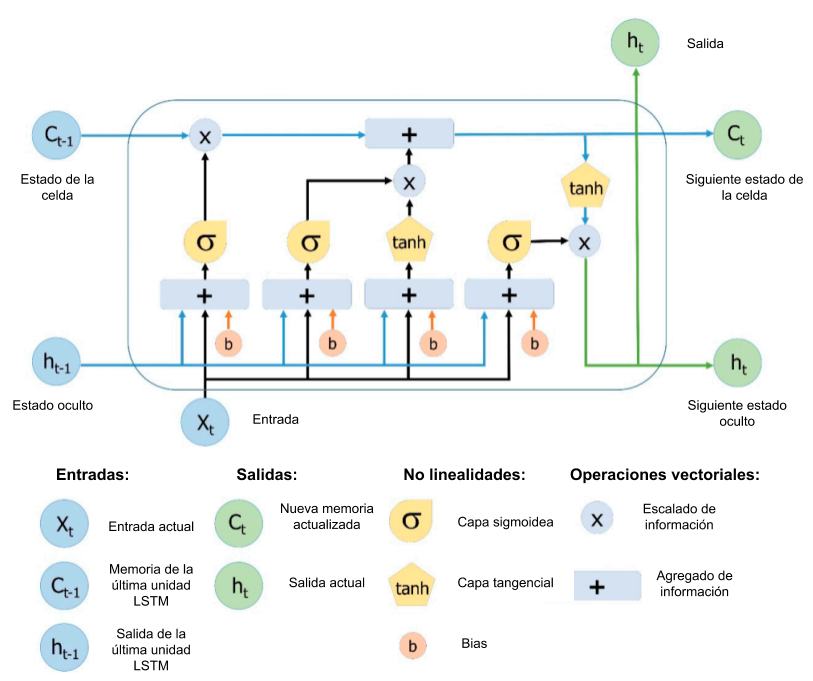
\includegraphics[width=0.95\textwidth, frame]{imagenes/Cap4/lstm}
  \caption{Estructura de LSTM. Reproducido desde Yan \protect\cite{Reference54}.} 
  \label{fig:lstm}
  \end{center}
\end{figure}

Una t\'{i}pica red LSTM esta compuesta por bloques de memoria llamados celdas. Dos estados se transfieren a la siguiente celda, el estado de la celda y el estado oculto. El \textbf{estado de la celda} es la cadena principal del flujo de datos, lo que permite que los datos fluyan hacia adelante, esencialmente, sin cambios. Sin embargo, pueden ocurrir algunas transformaciones lineales. Los datos pueden agregar o eliminar el estado de la celda a trav\'{e}s de puertas sigmoideas.

\vspace{5mm} %5mm vertical space

Una puerta es similar a una capa o una serie de operaciones matriciales, la cual contiene diferentes pesos individuales. Los LSTM est\'{a}n dise\~{n}ados para evitar el problema de dependencia a largo plazo porque utiliza puertas para controlar el proceso de memorizaci\'{o}n. 

\subsection{GRU}

GRU\footnote{\textbf{GRU, }Gated Recurrent Unit} fue dise\~{n}ado por primera vez por Kyunghyun Cho en \citeyear{Reference55}. Esta estructura de RNN s\'{o}lo contiene dos puertas. La puerta de actualizaci\'{o}n controla la informaci\'{o}n que fluye hacia la memoria, mientras que la puerta de reinicio controla la informaci\'{o}n que fluye fuera de la memoria. De manera similar a la LSTM, GRU tiene unidades de compuerta que modulan el flujo de informaci\'{o}n dentro de la unidad; sin embargo, sin tener una celda de memoria separada. Se podr\'{i}a decir que GRU es una variante de RNN un poco m\'{a}s simplificada que a menudo ofrece un rendimiento comparable a LSTM y es significativamente m\'{a}s r\'{a}pido de calcular.

\vspace{5mm} %5mm vertical space

En resumen, las GRU tienen las siguientes dos caracter\'{i}sticas distintivas:

\begin{itemize}
\item Las \textbf{puertas de reinicio} ayudan a capturar dependencias a corto plazo en series de tiempo.
\item Las \textbf{puertas de actualizaci\'{o}n} ayudan a capturar dependencias a largo plazo en series de tiempo.
\end{itemize}

\begin{figure}[h!]
  \begin{center}	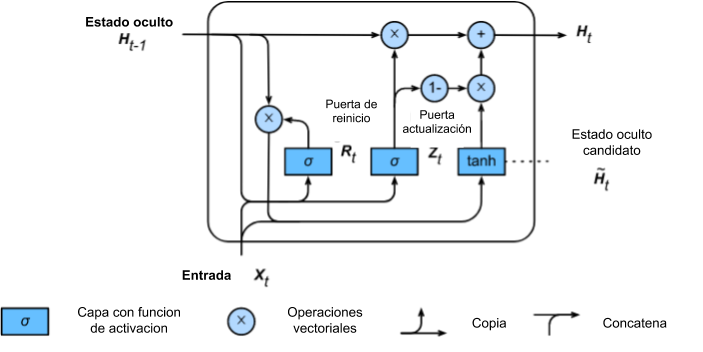
\includegraphics[width=0.95\textwidth, frame]{imagenes/Cap4/gru}
  \caption{Estructura de GRU. Reproducido desde \protect\cite{Reference56}.} 
  \label{fig:gru}
  \end{center}
\end{figure}


\section{T\'{e}cnicas de detecci\'{o}n de anomal\'{i}as}

Existen varios enfoques disponibles para la detección de anomalías, en esta secci\'{o}n se describir\'{a} algunos de los algoritmos m\'{a}s usados.

\subsection{One-Class SVM}

One-Class SVM\footnote{\textbf{SVM, }Support Vector Machine} (OC-SVM) es un enfoque ampliamente utilizado para descubrir anomal\'{i}as de forma no supervisada \cite{Reference59}. Las OC-SVM son una de las técnicas de aprendizaje semi-supervisado más utilizadas, debido a que da buenos resultados incluso para conjuntos de datos de alta dimensión. Sin embargo, este algoritmo tiene la desventaja de que requiere mucho tiempo y memoria en la práctica y su complejidad crece de forma cuadrática con el número de registros.

\vspace{5mm} %5mm vertical space

Este algoritmo s\'{o}lo se entrena con ejemplos positivos (clases normales). La idea general de \'{e}ste algoritmo es transformar el espacio de atributos y dibujar un hiperplano divisorio para que las observaciones se encuentren lo m\'{a}s lejos posible del origen, como se puede observar en la Figura \ref{fig:oc-svm}.

\begin{figure}[h!]
  \begin{center}	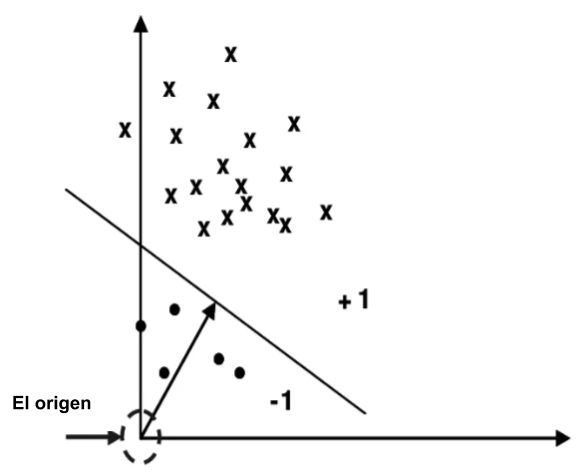
\includegraphics[width=0.45\textwidth, frame]{imagenes/Cap4/oc-svm}
  \caption{One-Class SVM. Reproducido desde \protect\cite{Reference72}} 
  \label{fig:oc-svm}
  \end{center}
\end{figure}

\vspace{5mm} %5mm vertical space

Como resultado, se obtiene un margen, en un lado del cual las observaciones de la muestra de entrenamiento se agrupan lo más densamente posible (observaciones normales $\hat{y_{i}} = 1$) , y en el otro, se encuentran los valores anormales ( $\hat{y_{i}} = -1$ ), no similares a lo que el algoritmo vi\'{o} durante el entrenamiento.


\subsection{Isolation Forest}

Este modelo se usa en un escenario similar al SVM de una clase, específicamente en un entorno no supervisado. El bosque de aislamiento adopta un enfoque diferente del SVM de una clase, ya que en lugar de agrupar datos normales, trata de aislar los datos anómalos.

\vspace{5mm} %5mm vertical space

El componente básico del Isolation Forest (Bosque de aislamiento) es el árbol de aislamiento, que es un árbol binario simple donde en cada nodo $T_{i}$ tanto la característica como el umbral para la regla de división se seleccionan aleatoriamente. Un nodo existente deja de generar hijos si y solo si solo hay un ejemplo siguiendo la regla de división para esa ruta específica (lo que significa que el ejemplo se ha aislado) o se ha alcanzado una altura máxima. Esto significa que al final del proceso de capacitación tendremos un árbol de clasificación aleatorio completamente sobreajustado, que puede usarse para fines de detección de anomalías. La intuición principal de este algoritmo es que si un ejemplo es anómalo, se aislará después de algunos cortes en el espacio de características, lo que se traduce en tener una baja altura en el árbol de aislamiento.

\vspace{5mm} %5mm vertical space

A diferencia de otros métodos como la agrupación o clasificación, los bosques de aislamiento no aprenden un perfil de lo que es normal, sino que atacan directamente las anomalías. No se utiliza métrica de distancia en este algoritmo lo cual ahorra tiempo en los cálculos; por lo que los bosques de aislamiento tienen una complejidad temporal lineal. 

\vspace{5mm} %5mm vertical space	

En la Figura \ref{fig:comparacion} se presenta una comparaci\'{o}n de la capacidad de los algoritmos Isolation Forest y One-Class SVM para hacer frente a diferentes conjuntos de datos de dos dimensiones, con el objetivo de dar cierta intuici\'{o}n acerca del comportamiento de estos algoritmos.

\begin{figure}[h!]
  \begin{center}	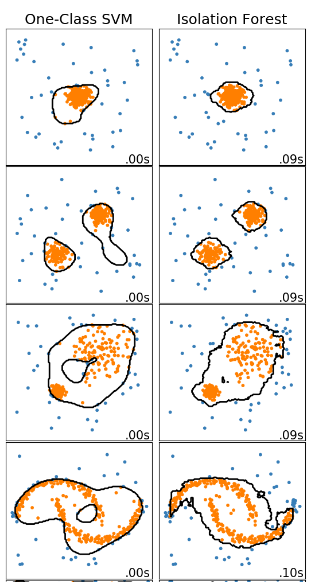
\includegraphics[width=0.43\textwidth, frame]{imagenes/Cap4/comp_if_ocsvm}
  \caption{Comparacion del rendimiento entre los algoritmos One-Clas SVM e Isolation Forest. Reproducido desde \protect\cite{Reference73}.} 
  \label{fig:comparacion}
  \end{center}
\end{figure}

\subsection{Autoencoders}

Hoy en día, los autoencoders se han utilizado ampliamente en la clasificación de imágenes, traducción automática y procesamiento de voz; esto debido a su capacidad de compresión de datos sin supervisión. Hasta donde se sabe, \shortciteA{Reference57} y \shortciteA{Reference58} fueron los primeros que propusieron autocodificadores para la detección de anomalías. Desde entonces, la capacidad de los autoencoders para detectar valores at\'{i}picos se demostró en diferentes dominios como por ejemplo la detecci\'{o}n de anomal\'{i}as en rayos X.

\vspace{5mm} %5mm vertical space

El m\'{e}todo tradicional de detecci\'{o}n de anomal\'{i}as basada en autoencoder se basa principalmente en el error de reconstrucci\'{o}n, considerando como anomal\'{i}as aquellas muestras que presentan un alto error de reconstrucci\'{o}n. En la fase de entrenamiento, solo se usan datos normales para entrenar el autoencoder, con el objetivo de minimizar el error de reconstrucci\'{o}n, de modo que el autoencoder pueda reconocer las caracter\'{i}sticas de los datos normales. En la fase de prueba, el autoencoder entrenado podr\'{a} reconstruir datos normales con peque\~{n}os errores de reconstrucci\'{o}n, pero fallar\'{a}n con datos an\'{o}malos que el autoencoder no ha encontrado antes y, por lo tanto, tienen errores de reconstrucci\'{o}n relativamente m\'{a}s altos en comparaci\'{o}n a los datos normales. Por lo tanto, al comparar si el puntaje de reconstrucci\'{o}n de una anomal\'{i}a est\'{a} por encima de un umbral (threshold) predefinido, el autoencoder determinar si los datos presentados para la prueba son an\'{o}malos \cite{Reference47} (Ver Figura \ref{fig:autoencoder-anomaly}). La ecuaci\'{o}n \ref{eqn:threshold} se observa como esta t\'{e}cnica determina lo que es una anomal\'{i}a y lo que no lo es; donde $S_{z}$ representa el error de reconstrucci\'{o}n.

\begin{equation}
C(z) = \left\lbrace
\begin{array}{ll}
\textup{si } S_{z}\leq \textup{Umbral} & \textup{Comportamiento normal}\\
\textup{si } S_{z}> \textup{Umbral} & \textup{Anomal\'{i}a}
\end{array}
\right.
\label{eqn:threshold}
\end{equation}

\begin{figure}[h!]
  \begin{center}	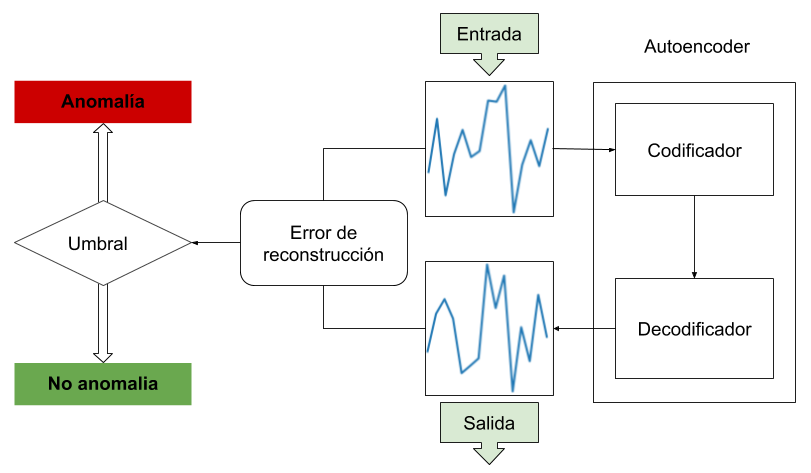
\includegraphics[width=0.95\textwidth, frame]{imagenes/Cap4/autoencoder-anomaly}
  \caption{Detecci\'{o}n de anomal\'{i}as con autoencoder (Elaboraci\'{o}n propia).} 
  \label{fig:autoencoder-anomaly}
  \end{center}
\end{figure}


\section{M\'{e}tricas de evaluaci\'{o}n}
%https://towardsdatascience.com/metrics-to-evaluate-your-machine-learning-algorithm-f10ba6e38234

Evaluar los algoritmos de aprendizaje autom\'{a}tico es una parte esencial para cualquier proyecto, debido a que un modelo puede brindar resultados satisfactorios cuando es evaluado con una m\'{e}trica; pero puede dar un resultado deficiente cuando se utiliza otra m\'{e}trica. Com\'{u}nmente se usa la precisi\'{o}n de clasificaci\'{o}n para medir el rendimiento de un modelo, sin embargo, no es suficiente para juzgar un modelo. A continuaci\'{o}n se cubrir\'{a} diferentes tipos de m\'{e}tricas de evaluaci\'{o}n.

\subsection{Precisi\'{o}n de clasificaci\'{o}n (accuracy)}

La precisi\'{o}n de clasificaci\'{o}n, conocida tambi\'{e}n con el nombre de precisi\'{o}n, es la relaci\'{o}n entre el n\'{u}mero de predicciones correctas y el n\'{u}mero total de muestras de entrada.

\begin{equation}
\textup{Precisi\'{o}n} = \frac{\textup{N\'{u}mero de predicciones correctas}}{\textup{N\'{u}mero total de predicciones realizadas}}
\end{equation}

Esta m\'{e}trica funciona bien si hay el mismo n\'{u}mero de muestras que pertenecen a cada clase; por ejemplo, si se considera que se tiene un conjunto de datos que contiene 98\% de muestras que pertenecen a la clase A y 2\% que pertenecen a la clase B, el modelo podr\'{i}a obtener f\'{a}cilmente un 98\% de precisi\'{o}n de entrenamiento simplemente prediciendo cada muestra de entrenamiento como clase A. 

\vspace{5mm} %5mm vertical space

Esto conlleva que la precisi\'{o}n puede dar la falsa sensaci\'{o}n de lograr una alta precisi\'{o}n, lo cual se convierte en un verdadero problema si se trata problemas que conllevan la detecci\'{o}n de cosas de alto riesgo; por ejemplo, de una enfermedad rara pero mortal ya que el costo de no diagnosticar la enfermedad de una persona enferma es mucho mayor que el costo de enviar a una persona sana a realizarce  m\'{a}s an\'{a}lisis.

\subsection{P\'{e}rdida logar\'{i}tmica (Logarithmic Loss)}

La p\'{e}rdida logar\'{i}tmica, conocida tambi\'{e}n como \textit{Log Loss}, funciona penalizando las clasificaciones falsas, adem\'{a}s tiene un buen rendimiento para la clasificaci\'{o}n de varias clases. Cuando se trabaja con Log Loss, el clasificador debe asignar una probabilidad a cada clase de todas las muestras; suponiendo que hay $N$ muestras que pertenecen a clases $M$, Log Loss se calcula seg\'{u}n la siguiente ecuaci\'{o}n:

\begin{equation}
LogarithmicLoss = \frac{-1}{N}\sum_{i=1}^{N}\sum_{j=1}^{M} y_{ij}*log(p_{ij})
\end{equation}

donde:
\\
$y_{ij}$, indica si la muestra $i$ pertenece a la clase $j$ o no.\\
$p_{ij}$, indica la probabilidad de que la muestra $i$ pertenezca a la clase $j$.

\vspace{5mm} %5mm vertical space

Log Loss no tiene l\'{i}mite superior y existe en el rango $[0, \infty )$. Cuando se obtiene un Log Loss cercano a 0 indica una mayor precisi\'{o}n, mientras que si est\'{a} lejos de 0 indica una menor precisi\'{o}n. En general se puede decir que minimizar Log Loss proporciona una mayor precisi\'{o}n para el clasificador.

\subsection{Matriz de confusi\'{o}n}

La matriz de confusi\'{o}n, tambi\'{e}n llamada matriz de error, es el m\'{e}todo m\'{a}s com\'{u}n para evaluar la exactitud de un resultado de clasificaci\'{o}n \cite{Reference61}. Esta matriz es una tabulaci\'{o}n cruzada de los datos esperados y los resultados de la clasificaci\'{o}n del modelo. El n\'{u}mero de columnas y filas es igual al n\'{u}mero de categor\'{i}as de las clasificaci\'{o}n y de ellas se derivan diferentes medidas estad\'{i}sticas.

\begin{table}[H]

\centering
\begin{center}
\begin{tabular}{ll|c|c|}
\cline{3-4}
                                                        &                                              & \multicolumn{2}{c|}{\textbf{Predicci\'{o}n}}                                                          \\ \cline{3-4} 
                                                        &                                              & \textbf{Clase Positiva}                         & \textbf{Clase Negativa}                         \\ \hline
\multicolumn{1}{|c|}{}                                  & \multicolumn{1}{c|}{\textbf{Clase Positiva}} & \cellcolor[HTML]{AADD99}Verdadero Positivo (VP) & \cellcolor[HTML]{FFCE93}Falso Negativo (FN)     \\ \cline{2-4} 
\multicolumn{1}{|c|}{\multirow{-2}{*}{\textbf{Reales}}} & \multicolumn{1}{c|}{\textbf{Clase Negativa}} & \cellcolor[HTML]{DF9F9F}Falso Positivo (FP)     & \cellcolor[HTML]{AADD99}Verdadero Negativo (VN) \\ \hline
\end{tabular}
\caption{Matriz de confusi\'{o}n, para una clasificaci\'{o}n binaria (Elaboraci\'{o}n propia).}
\label{table:matriz}
\end{center}
\end{table}

\vspace{5mm} %5mm vertical space

En el Cuadro \ref{table:matriz} las filas de la matriz representan los valores reales, mientras que las columnas est\'{a}n asociadas con los datos clasificados por el modelo (predicciones). La diagonal principal, que se presenta de color verde, indica los aciertos \'{o} Verdaderos Positivos (VP) y Verdaderos Negativos (VN), que son todos aquellos datos donde el modelo obtiene el mismo resultado que se esperaba obtener. En cuanto a todos los dem\'{a}s valores de la matriz pertenecen a aquellos datos que fueron clasificados de forma err\'{o}nea, estos se clasifican en dos clases: Falsos Positivos (FP), que en la matriz se presentan de color rojo y Falsos Negativos (FN) que en la matriz fueron representados de color naranja.

\vspace{5mm} %5mm vertical space

La precisi\'{o}n global de la matriz se calcula dividiendo la suma de muestras correctamente clasificadas por el n\'{u}mero total de muestras tomadas \ref{eqn:exactitud}. Este valor es una medida de clasificaci\'{o}n como un todo, ya que indica la probabilidad de que una muestra se clasifique correctamente.

\begin{equation}
Exactitud=\frac{VP+VN}{VP+VN+FP+FN}
\label{eqn:exactitud}
\end{equation}

La exactitud no es una medida adecuada para la evaluaci\'{o}n de algoritmos de detecci\'{o}n de valores at\'{i}picos, debido a que la mayoria de las veces un falso negativo es mucho m\'{a}s costoso que un falso positivo, adem\'{a}s que los conjuntos de entrenamiento presentan una gran cantidad de datos normales comparado a la cantidad de datos an\'{o}malos. Existen dos m\'{e}tricas comunes para evaluar algoritmos de detecci\'{o}n de valores at\'{i}picos, AUC y F1 Score; a continuaci\'{o}n se profundizar\'{a} detalladamente estas dos m\'{e}tricas.

\subsection{\'{A}rea bajo la curva (AUC)}

\'{A}rea bajo la curva (AUC\footnote{\textbf{AUC, }Area Under Curve}) es una de las m\'{e}tricas m\'{a}s utilizadas para la evaluaci\'{o}n. Se utiliza para problemas de clasificaci\'{o}n binaria.

\vspace{5mm} %5mm vertical space

El AUC de un clasificador es igual a la probabilidad de que el clasificador clasifique un ejemplo positivo elegido al azar m\'{a}s alto que un ejemplo negativo elegido al azar. Antes de definir AUC, se debe comprender los siguientes t\'{e}rminos:

\subsubsection{Tasa de Verdaderos Positivos (TPR)}

La tasa de verdaderos positivos (TPR\footnote{\textbf{TPR, }de sus siglas en ingl\'{e}s True Positive Rate, tambi\'{e}n conocido como Sensitivity.}), tambi\'{e}n conocida como sensibilidad, corresponde a la proporción de puntos de datos positivos que se consideran correctamente como positivos, con respecto a todos los puntos de datos positivos. Se define seg\'{u}n la ecuaci\'{o}n \ref{eqn:sensibility}.

\begin{equation}
Sensibilidad = \frac{VP}{FN+VP}
\label{eqn:sensibility}
\end{equation}

\subsubsection{Tasa de Falsos Positivos (FPR) }

La tasa de falsos positivos (FPR\footnote{\textbf{FPR, }de sus siglas en ingl\'{e}s False Positive Rate, tambi\'{e}n conocido como Specificity.}), tambi\'{e}n conocida como especificidad, corresponde a la proporción de puntos de datos negativos que se consideran erróneamente como positivos, con respecto a todos los puntos de datos negativos. Se define seg\'{u}n la ecuaci\'{o}n \ref{eqn:specificity}.

\begin{equation}
Especificidad = \frac{FP}{FP+VN}
\label{eqn:specificity}
\end{equation}

\subsubsection{ROC (Receiver Operating Characteristics)}

ROC es la curva dibujada conectando los puntos del eje X = FPR (Tasa de falsos positivos) y el eje y = TPR (Tasa de verdaderos positivos) para diferentes valores de un umbral de discriminaci\'{o}n (l\'{i}mite de decisi\'{o}n para determinar si un valor corresponde a una clase o no) para un modelo, es decir, se elige diferentes umbrales para un modelo, se calcula el TPR y FPR para cada umbral, luego dibuja la curva ROC y finalmente se calcula el AUC, que es el \'{a}rea bajo la curva ROC. En la Figura \ref{fig:auc_roc} se muestra un ejemplo de la curva AUC-ROC.

\begin{figure}[h!]
  \begin{center}	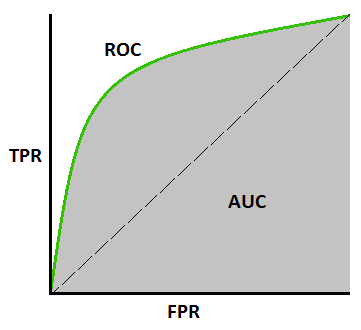
\includegraphics[width=0.65\textwidth, frame]{imagenes/Cap4/auc_roc}
  \caption{Ejemplo de un curva AUC-ROC \protect\cite{Reference62}.}
  \label{fig:auc_roc}
  \end{center}
\end{figure}


\vspace{5mm} %5mm vertical space

Existen dos razones principales por lo que se necesita esta curva, la primera es que refleja que tan bueno es el modelo para separar dos clases y la segunda es que ayuda a elegir el mejor umbral; por ejemplo, un AUC igual a 0,5 significa que el modelo separa dos posibles resultados al azar y un AUC de 1 (valor m\'{a}ximo) implica una separaci\'{o}n perfecta; por lo tanto se puede decir que mientras mayor sea el valor de AUC mejor es el rendimiento del modelo que se este evaluando.

\subsection{F1 Score}

F1 Score define que tan preciso es un modelo, es decir, cu\'{a}ntas instancias clasifica correctamente, as\'{i} como tambi\'{e}n indica que tan robusto es el modelo. Esta m\'{e}trica es necesaria cuando se desea buscar un equilibrio entre la precisi\'{o}n y la recuperaci\'{o}n, ya que da una evaluaci\'{o}n justa incluso cuando el conjunto de datos se encuentra desequilibrado.

\subsubsection{Precisi\'{o}n (Precision)}

La precisi\'{o}n es el n\'{u}mero de resultados positivos correctos dividido por el n\'{u}mero de resultados positivos predichos por el clasificador.

\begin{equation}
Precision = \frac{VP}{VP+FP}
\end{equation}

\subsubsection{Recuperaci\'{o}n (Recall)}

Es el n\'{u}mero de resultados positivos correctos dividido por el n\'{u}mero de todas las muestras que deber\'{i}an haber sido clasificadas como positivas.

\begin{equation}
Recall = TPR = \frac{VP}{VP+FN}
\end{equation}

Por lo tanto, F1 Score se expresa matem\'{a}ticamente como:

\begin{equation}
F1 = 2*\frac{1}{\frac{1}{Precision}+\frac{1}{Recall}}
\end{equation}

%\section{Resumen del cap\'{i}tulo}

%Este cap\'{i}tulo detalla las bases te\'{o}ricas, permitiendo complementar los conocimientos necesarios para abordar el desarrollo del m\'{e}todo de detecci\'{o}n de anomal\'{i}as de conducci\'{o}n mediante el uso de Aprendizaje Autom\'{a}tico. En primer lugar, se decribi\'{o} los diferentes paradigmas de aprendizaje que existen y los diferentes enfoques de modelos, luego, se realiz\'{o} una descripci\'{o}n del funcionamiento de las redes neuronales y se mostr\'{o} sus diferentes tipos, as\'{i} como tambi\'{e}n diferentes t\'{e}cnicas de detecci\'{o}n de anomal\'{i}as y por \'{u}timo se presenta diferentes m\'{e}tricas de evaluaci\'{o}n de modelos de aprendizaje autom\'{a}tico. 

%El siguiente cap\'{i}tulo detalla el proceso de captura y preparaci\'{o}n del conjunto de datos, una etapa importante, debido a que este conjunto ser\'{a} aquel con el que se entrenar\'{a} el mecanismo de detecci\'{o}n de anomal\'{i}as propuesto.

El siguiente cap\'{i}tulo detalla el proceso de captura y preparaci\'{o}n del conjunto de datos, una etapa importante, debido a que este conjunto ser\'{a} aquel con el que se entrenar\'{a} el mecanismo de detecci\'{o}n de anomal\'{i}as propuesto.
